\section{Experiments}

\begin{table*}[t!]
    \centering
    \caption{Performance (F1 scores) comparison of various retrieval methods across different tasks, with all models evaluated using \textit{Llama-3.3-70B-Instruct} as the backbone. Results are directly reported from HippoRAG2 \cite{gutierrez2025rag} by default, while methods marked with ($^*$) denote our local reproduction. The best results are in \textbf{bold}, and the second best are \underline{underlined}. The $^\dagger$ symbol indicates a failure in graph construction due to large corpus size.}    \label{tab:results}
    \small
    \vspace{-5pt}
%    \resizebox{\textwidth}{!}{
    \begin{tabular}{l cccccc c}
        \toprule
        & \multicolumn{2}{c}{Simple QA} & \multicolumn{4}{c}{Multi-Hop QA} & \\
        \cmidrule(lr){2-3} \cmidrule(lr){4-7}
        Retrieval & NQ & PopQA & MuSiQue & 2Wiki & HotpotQA & LV-Eval & Avg \\
        \midrule
        \multicolumn{8}{c}{\textit{Simple Baselines}} \\
        \midrule
        None & 54.9 & 32.5 & 26.1 & 42.8 & 47.3 & 6.0 & 34.9 \\
        Contriever \cite{izacard2021unsupervised} & 58.9 & 53.1 & 31.3 & 41.9 & 62.3 & 8.1 & 42.6 \\
        BM25 \cite{robertson1994some} & 59.0 & 49.9 & 28.8 & 51.2 & 63.4 & 5.9 & 43.0 \\
        GTR \cite{ni2022large} & 59.9 & 56.2 & 34.6 & 52.8 & 62.8 & 7.1 & 45.6 \\
        \midrule
        \multicolumn{8}{c}{\textit{Large Embedding Models}} \\
        \midrule
        GTE-Qwen2-7B \cite{ni2022large} & 62.0 & 56.3 & 40.9 & 60.0 & 71.0 & 7.1 & 49.6 \\
        GritLM-7B \cite{muennighoff2024generative} & 61.3 & 55.8 & 44.8 & 60.6 & 73.3 & 9.8 & 50.9 \\
        NV-Embed-v2 \cite{lee2024nv} & 61.9 & 55.7 & 45.7 & 61.5 & 75.3 & 9.8 & 51.7 \\
        \midrule
        \multicolumn{8}{c}{\textit{Graph-based RAG Methods}} \\
        \midrule
        RAPTOR \cite{sarthi2024raptor} & 50.7 & 56.2 & 28.9 & 52.1 & 69.5 & 5.0 & 43.7  \\
        GraphRAG \cite{edge2024local} & 46.9 & 48.1 & 38.5 & 58.6 & 68.6 & 11.2 & 45.3 \\
        LightRAG \cite{guo2024lightrag} & 16.6 & 2.4 & 1.6 & 11.6 & 2.4 & 1.0 & 5.9 \\
        HippoRAG \cite{jimenez2024hipporag} & 55.3 & 55.9 & 35.1 & 71.8 & 63.5 & 8.4 & 48.3 \\
        HippoRAG2 \cite{gutierrez2025rag} & \underline{63.3} & \underline{56.2} & \textbf{48.6} & \underline{71.0} & \underline{75.5} & \textbf{12.9} & \underline{54.6} \\
        % HippoRAG2$^*$ \cite{gutierrez2025rag} & 62.5 & 55.7 & \textbf{48.7} & \underline{71.6} & 75.3 & 10.9 & 54.1 \\
        LinearRAG$^*$ \cite{zhuang2025linearrag} & 54.5 & 26.0 & 31.0 & 54.9 & 59.0 & 10.3 & 39.3 \\
        HyperGraphRAG$^*$ \cite{luo2025hypergraphrag} & 53.6 & 26.4 & 41.6 & 61.2 & 73.1 & N/A$^\dagger$ & - \\
        \midrule
        \rowcolor{blue!10} \textbf{HELP (Ours)} & \textbf{63.5} & \textbf{57.6} & \underline{48.4} & \textbf{73.9} & \textbf{75.6} & \underline{12.5} & \textbf{55.3} \\
        \bottomrule
    \end{tabular}
\vspace{-5pt}
\end{table*}

We conduct comprehensive experiments to verify the accuracy and efficiency of HELP across a diverse range of single-hop and multi-hop QA benchmarks. By comparing HELP against traditional dense retrievers, embedding models, and current Graph-based RAG frameworks, we aim to demonstrate its superior ability to localize high-quality evidence. Furthermore, we provide in-depth ablation studies to validate our Hypernode Expansion and Logical Path-Guided Evidence Localization Strategies.
\subsection{Experimental Settings}

\textbf{Datasets.} 
%We follow the setup and datasets established in HippoRAG2 \cite{gutierrez2025rag}. 
Our evaluation spans both Simple QA and Multi-Hop QA tasks to ensure a comprehensive assessment. For Simple QA, we utilize NaturalQuestions (NQ) dataset \cite{wang2024rear} and PopQA \cite{mallen-etal-2023-trust}; for the more challenging Multi-Hop QA, we include MuSiQue \cite{trivedi-etal-2022-musique}, 2WikiMultiHopQA(2Wiki) \cite{ho2020constructing}, HotpotQA \cite{yang2018hotpotqa}, and LV-Eval \cite{yuan2024lv}. By adopting identical data splits, corpora, and evaluation protocols as HippoRAG2~\cite{gutierrez2025rag}, we ensure a rigorous and fair comparison across both retrieval quality and generation accuracy.

\textbf{Baselines.} We compare HELP against a comprehensive set of baselines categorized into three groups, following the experimental protocol established by HippoRAG2 \cite{gutierrez2025rag}. First, we include classic and dense retrieval methods, namely BM25 \cite{robertson1994some}, Contriever \cite{izacard2021unsupervised}, and GTR \cite{ni2022large}. Second, we evaluate against state-of-the-art 7B-parameter embedding models that lead the BEIR benchmark\cite{thakur2021beir}, including GTE-Qwen2-7B-Instruct \cite{li2023towards}, GritLM-7B \cite{muennighoff2024generative}, and NV-Embed-v2 \cite{lee2024nv}. Finally, we compare HELP with Graph-based RAG methods, encompassing hierarchical approaches like RAPTOR \cite{sarthi2024raptor}, global summarization methods such as GraphRAG \cite{edge2024local} and LightRAG \cite{guo2024lightrag}, and knowledge-graph-based frameworks like HippoRAG \cite{jimenez2024hipporag}. For these aforementioned baselines, we directly report the results published in HippoRAG2 as they share an identical evaluation setting with our work. Furthermore, to ensure a timely and rigorous comparison, we faithfully reproduce the most recent advancements, including LinearRAG \cite{zhuang2025linearrag}, and HyperGraphRAG \cite{luo2025hypergraphrag}, under the same configurations to maintain complete experimental parity.

\textbf{Evaluation Metrics.} 
Consistent with the evaluation settings in HippoRAG \cite{jimenez2024hipporag} and HippoRAG2 \cite{gutierrez2025rag}, we employ the token-level F1 metric defined in the MuSiQue \cite{trivedi-etal-2022-musique}.

\textbf{Implementations.} For the implementation of HELP, we maintain strict architectural parity with the settings described in HippoRAG2 \cite{gutierrez2025rag} to ensure the validity of our comparative analysis. Specifically, \textit{Llama-3.3-70B-Instruct} \cite{llama3modelcard} powers both the knowledge extraction (NER/OpenIE) and response generation phases, while \textit{NV-Embed-v2} \cite{lee2024nv} serves as the primary retriever to bridge structural knowledge with semantic embeddings. Our QA module uses the top-5 retrieved passages as context for an LLM to generate the final answer. This same combination of extractor and retriever is applied across all reproduced Graph-based RAG baselines to ensure a fair evaluation.

\subsection{QA performance}
Table~\ref{tab:results} shows the performance of HELP compared to competitive baselines. The hyperparameter configurations for HELP are consistently applied across all datasets as detailed in Appendix~\ref{appendix: hyperparameter setting}. Overall, HELP sets a new state-of-the-art across the evaluated benchmarks, achieving a consistent performance gain over Graph-based RAG methods.

\textbf{Overall Superiority.} Compared to the previous leading Graph-based RAG method HippoRAG2, HELP yields a relative improvement of 1.3\% in average F1 score. Furthermore, HELP significantly outperforms the strongest large-scale embedding model NV-Embed-v2, with a 7.0\% relative gain in average F1, demonstrating that even state-of-the-art 7B embedding models can be significantly enhanced through our structural knowledge integration. When compared to traditional dense retrievers such as GTR, our method exhibits a substantial performance leap of 21.3\%, underscoring the vital necessity of bridging structural knowledge with semantic retrieval for complex question answering.

\begin{figure}[t!] % [t] 表示将图片置于页面顶部，[h] 为当前位置，[b] 为底部
    \centering
    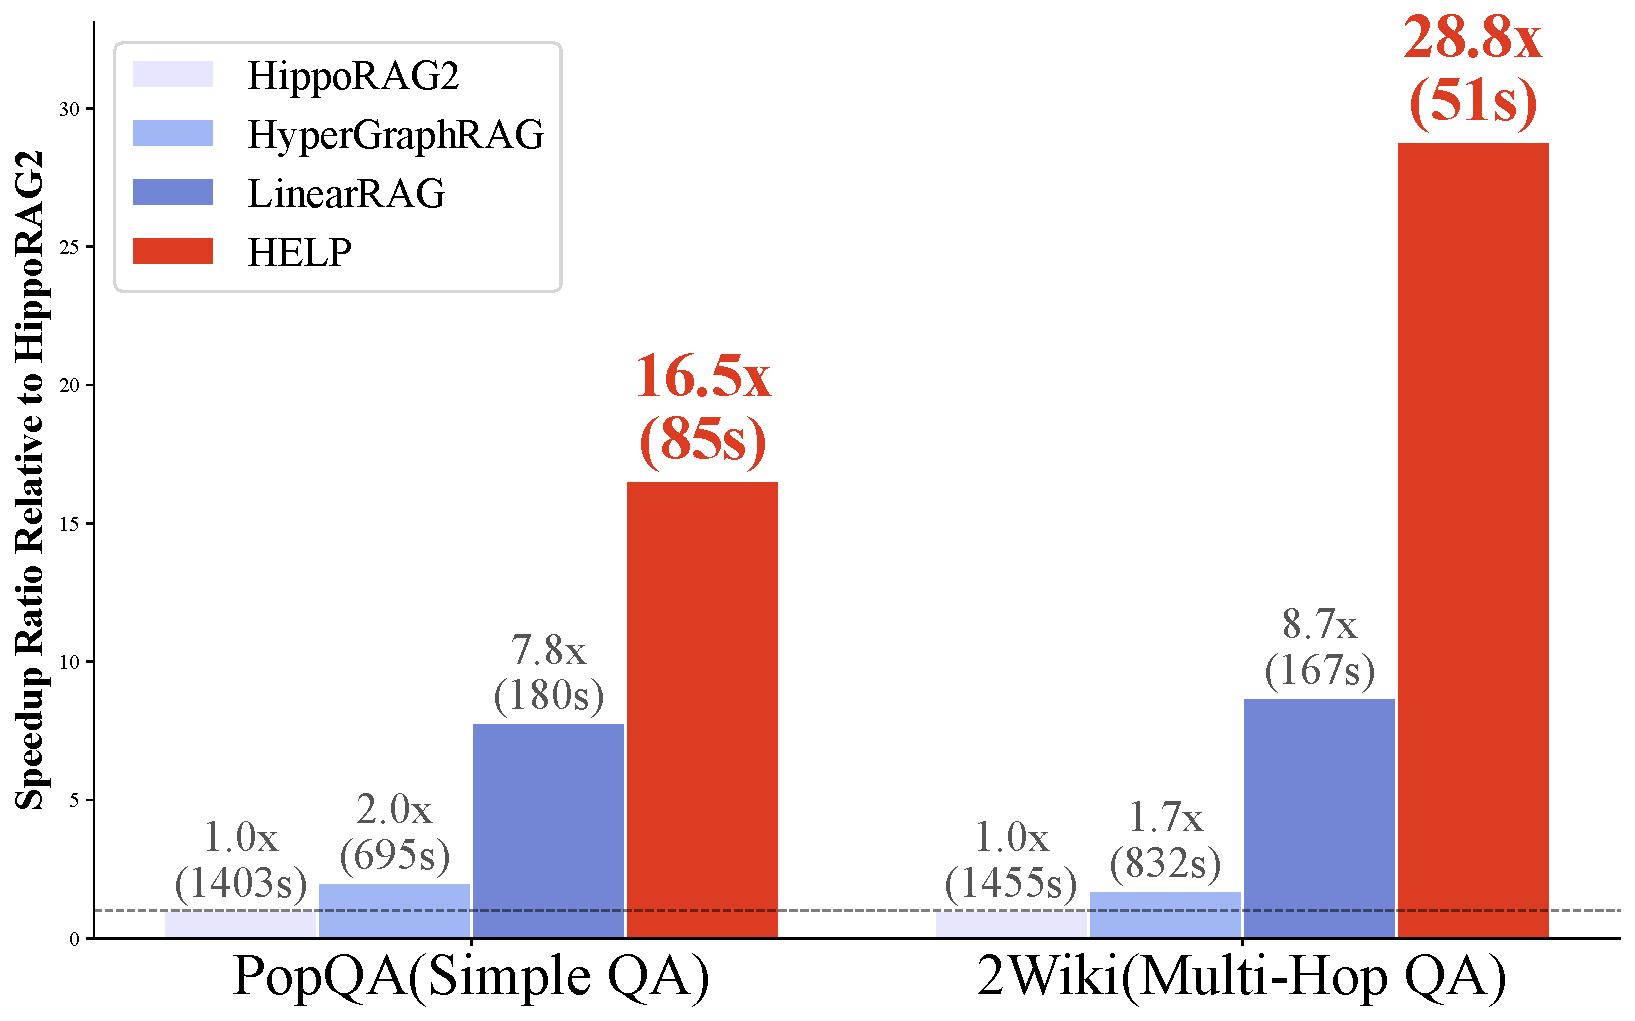
\includegraphics[width=1\linewidth]{figures/speedup_comparison_with_seconds.pdf} 
    \vspace{-18pt}
    \caption{Retrieval efficiency on PopQA (Simple QA) and 2Wiki (Multi-Hop QA). Absolute retrieval time (in seconds) for processing 1,000 queries are annotated above the bars, highlighting that HELP reduces the total retrieval latency to under 90 seconds.}
    \label{fig:speedup_comparison}
    \vspace{-10pt}
\vspace{-8pt}
\end{figure}

\textbf{Performance on Simple QA.} In single-hop scenarios represented by NQ and PopQA, HELP demonstrates superior retrieval precision. While the Hypernode Expansion mechanism is specifically engineered to navigate high-order relational dependencies in multi-hop reasoning, it notably maintains a competitive advantage in simpler, factoid-based tasks. Specifically, HELP achieves a 2.5\% relative improvement over the second-best performing method HippoRAG2 on PopQA dataset. Furthermore, it maintains a steady gain of 2.6\% to 3.4\% over the strongest 7B embedding models, such as NV-Embed-v2. This indicates that our knowledge-enhanced approach effectively anchors semantic search with precise evidence localization, ensuring that simple factoid queries benefit from the structural clarity of the knowledge graph while maintaining a decisive competitive edge over purely latent-space representations.

\textbf{Performance on Multi-Hop QA.} The advantages of HELP are most pronounced in complex reasoning tasks where relational dependencies are critical. On the 2Wiki dataset, HELP outperforms HippoRAG2 by 4.1\%. Compared to more recent methods like LinearRAG, HELP achieves a staggering 34.6\% relative improvement on the same benchmark, suggesting that our method more effectively navigates multi-hop paths than linear structures. Notably, while the indexing complexity of HyperGraphRAG rendered it unusable for the large-scale corpora of LV-Eval, HELP successfully processed the entire dataset, demonstrating both great reasoning capabilities and superior scalability.

\subsection{Retrieval Efficiency}

As illustrated in Fig.~\ref{fig:speedup_comparison}, we evaluated the retrieval time of HELP against three strong baselines: HippoRAG2, HyperGraphRAG, and LinearRAG.

Our method demonstrates overwhelming efficiency across both simple and multi-hop QA benchmarks. Specifically, on the PopQA dataset, HELP achieves a 16.5$\times$ speedup relative to HippoRAG2, drastically compressing the total retrieval time for 1,000 queries from 1,403s to a mere 85s. This performance gap widens even further on the complex 2Wiki dataset, where HELP attains a remarkable 28.8$\times$ speedup. Traditional graph-based baselines still suffer from the combinatorial explosion of graph traversals, requiring over 20 minutes to resolve dependencies, whereas HELP consistently completes the same tasks in under 90 seconds.

The significant efficiency gain of HELP stems from its HyperNode-based pruning strategy and a purely embedding-driven retrieval process. Unlike iterative graph methods that rely on LLMs for intermediate node filtering or path expansion, HELP bypasses these costly generative steps and the redundant neighbor explorations typical of traditional graph walks. Even when compared to LinearRAG, which was specifically designed to mitigate graph overhead, HELP further accelerates the process by approximately 2-3$\times$. This confirms that HELP successfully retains the structural reasoning benefits of knowledge graphs without succumbing to their traditional computational bottlenecks, proving its scalability for large-scale scenarios.


\begin{table}[t!]
\centering
\caption{Ablation study of the Hybrid Retrieval Strategy on the 2Wiki dataset. 
$M$ denotes the primary quota of passages assigned to the logical path-guided retrieval, while the total context size is fixed at 5. $M=0$ corresponds to a purely dense retrieval baseline.
}
\vspace{-5pt}
\label{tab:hybrid_ablation}
\small
\setlength{\tabcolsep}{12pt} % 增加列与列之间的间距
\begin{tabular}{c c c c}
\toprule
\textbf{Quota(M)} & \textbf{EM(\%)} & \textbf{F1(\%)} &  \textbf{Recall@5(\%)} \\
\midrule
0 & 57.5 & 61.55 & 76.25 \\
1 & 57.7 & 62.19 & 76.52 \\
2 & 63.0 & 69.52 & 84.95 \\
3 & 64.3 & 71.01 & 89.00 \\
\rowcolor{blue!10} \textbf{4} & \textbf{66.6} & \textbf{73.90} & \textbf{92.15} \\
5 & 65.9 & 73.09 & 91.65 \\
\bottomrule
\end{tabular}
\vspace{-20pt}
\end{table}

\subsection{Ablation Study}

\textbf{1) Hybrid Retrieval Strategy. }\label{sec: hybrid strategy}
Table~\ref{tab:hybrid_ablation} underscores the synergy between structural precision and semantic coverage within our Hybrid Retrieval Strategy. To provide a multi-dimensional assessment, we report both Exact Match (EM), which measures the percentage of predicted answers that exactly match the ground truth, and Recall@5, which indicates whether at least one of the top-5 retrieved passages contains the gold evidence required to answer the query. The evaluation shows that performance peaks at $M=4$, a 20\%+ improvement over pure dense retrieval ($M=0$), proving that logical paths effectively resolve multi-hop dependencies. However, when semantic backfill is constrained ($M=5$), performance slightly declines. This non-monotonic trend suggests that a purely logical path-guided approach is vulnerable to graph incompleteness and structural noise; thus, maintaining a dense retrieval component is essential as a robust fallback to ensure comprehensive evidentiary support.
 
% When $M=0$ (purely dense retrieval), it achieves an F1 of 61.55 and a Recall@5 of 76.25. As $M$ increases, performance surges significantly, peaking at $M=4$ with an F1 of 73.90 and a Recall@5 of 92.15. This represents a relative improvement of over 20\% in both metrics, indicating that logical path-guided localization effectively resolves complex multi-hop dependencies that remain ambiguous in pure semantic embeddings.
  
% Notably, performance slightly declines at $M=5$ when the semantic backfill is entirely omitted. This non-monotonic trend reveals a vital synergy: while the logical path provides high-precision structural anchors, the dense component serves as a robust fallback against graph incompleteness. These results empirically justify our Hybrid Retrieval Strategy is essential for achieving superior performance in multi-hop reasoning tasks.

% Table~\ref{tab:hybrid_ablation} underscores the synergy between structural precision and semantic coverage within our Hybrid Retrieval Strategy. 

\begin{figure}[t]
    \centering
    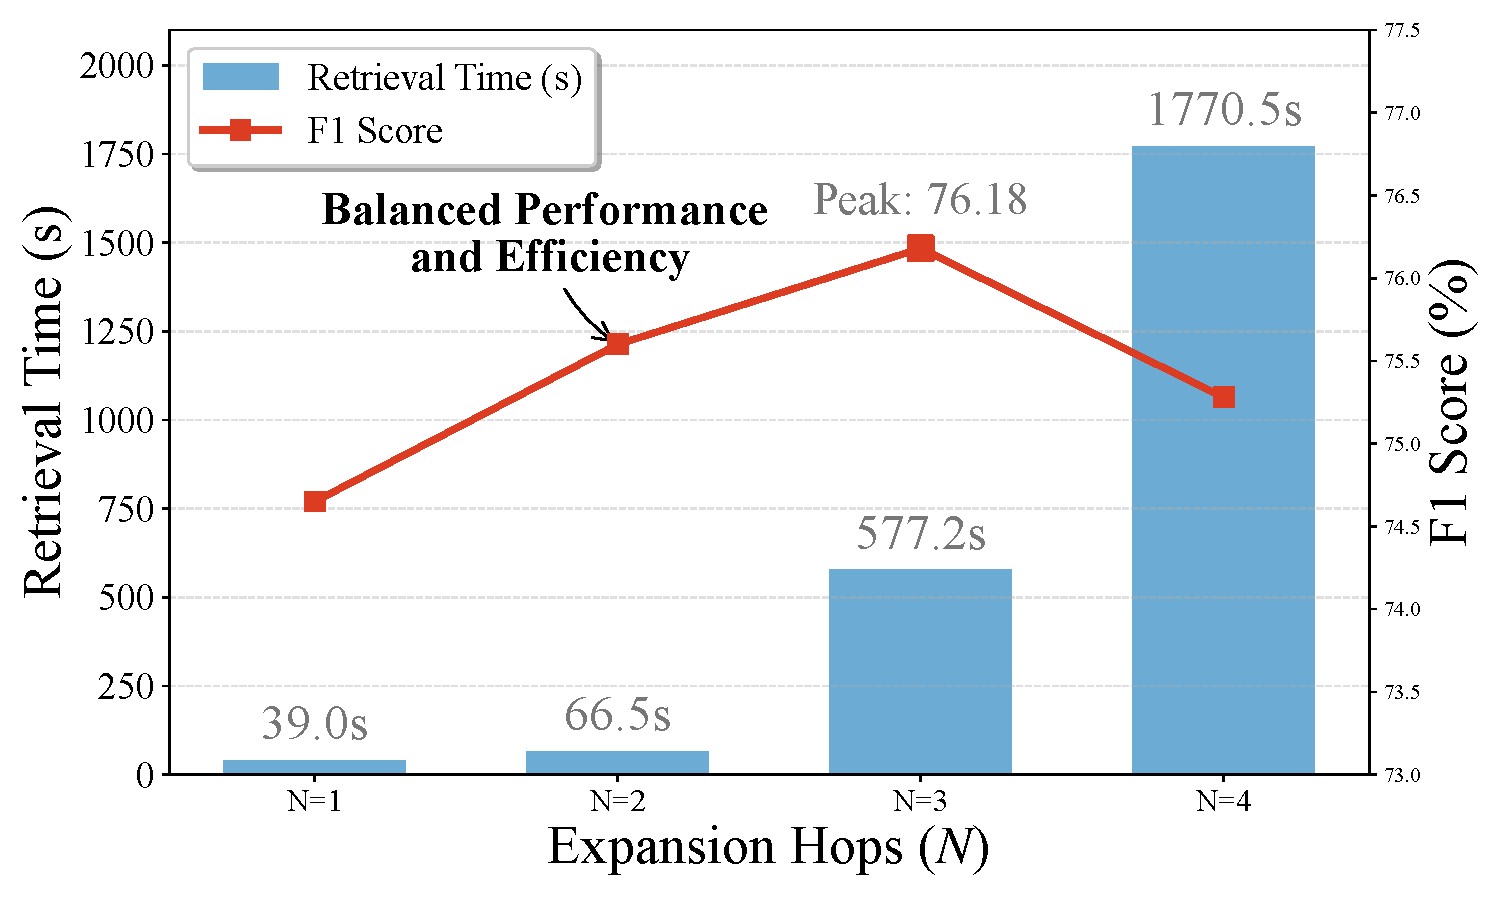
\includegraphics[width=1.0\linewidth]{figures/expansion_hops.pdf}
    \vspace{-18pt}
    \caption{Experimental analysis of expansion hops $N$ on HotpotQA dataset. The bars indicate retrieval time (left axis), while the line tracks the QA F1 score (right axis). }
    \label{fig:efficiency_bar_line}
\vspace{-15pt}
\end{figure}


\textbf{2) Impact of Expansion Hops.}
To investigate the trade-off between retrieval latency and QA performance, we conducted an ablation study on the number of expansion hops, denoted as $N$. In Fig.~\ref{fig:efficiency_bar_line}, varying $N$ reveals a significant divergence between computational cost and QA performance.

On one hand, the retrieval time exhibits an exponential growth pattern. While the latency remains manageable at $N=1$ and $N=2$, it surges dramatically to $577.2$s at $N=3$ and becomes prohibitive at $N=4$. On the other hand, the F1 score follows a non-monotonic trajectory, yet remarkably remains above $74.5\%$ across all values of $N$, demonstrating HELP's robustness and strong performance. Specifically, performance peaks at $76.18\%$ when $N=3$, as deeper exploration retrieves more relevant context. However, increasing $N$ to $4$ leads to a performance degradation. This decline suggests that excessive expansion introduces significant noise and irrelevant information, which outweighs the benefits of broader context coverage. Given that the F1 score remains competitive even at lower hops, $N=2$ offers a compelling balance, achieving high accuracy with only a fraction of the computational overhead required for $N=3$.


\begin{figure}[t]
    \centering
    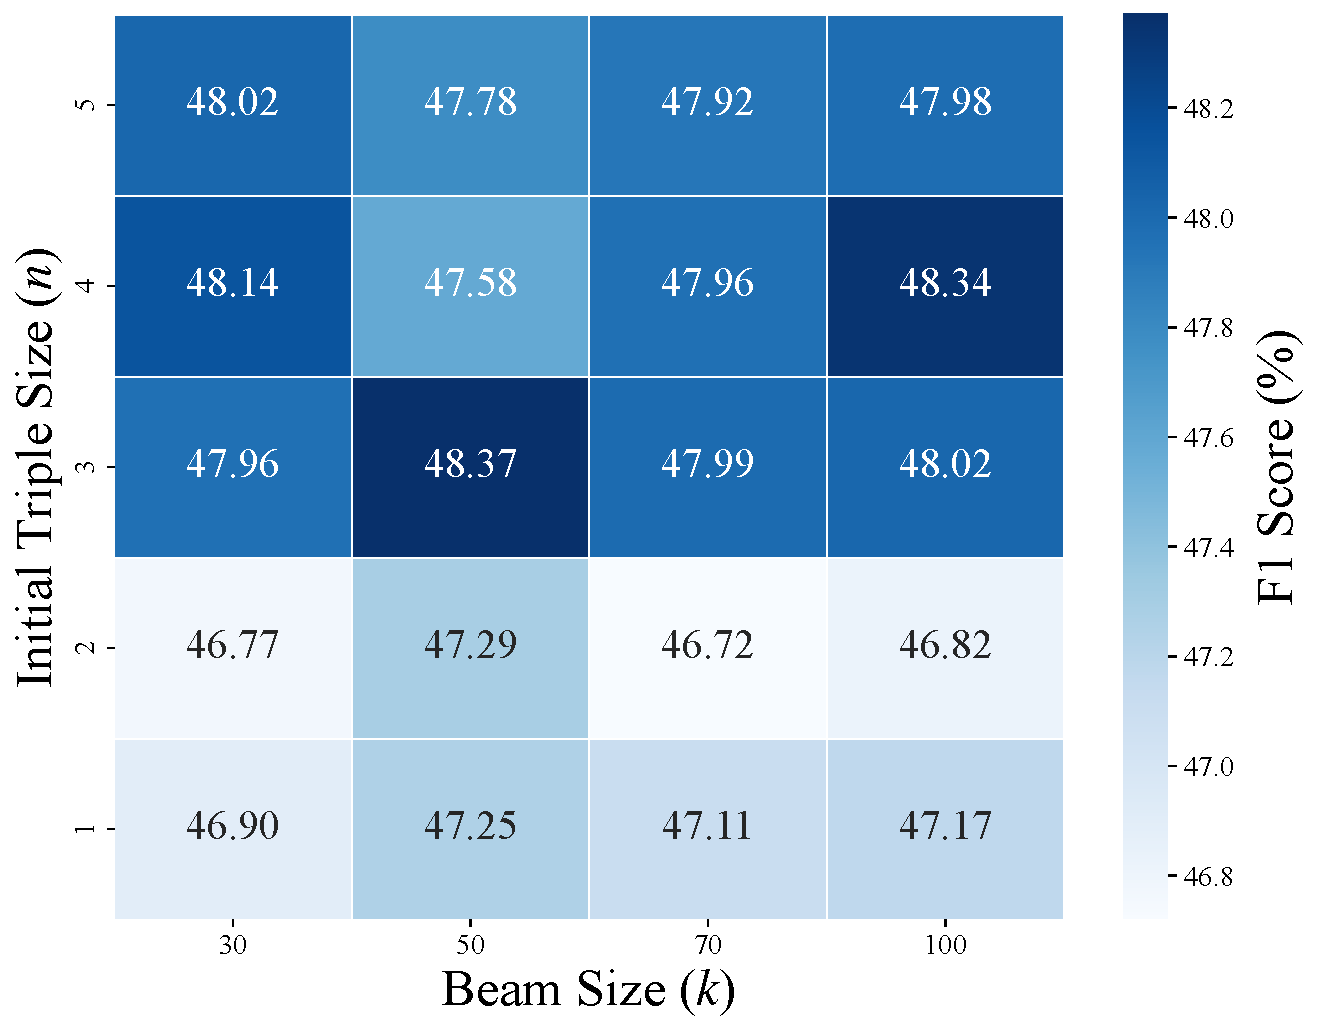
\includegraphics[width=0.9\linewidth]{figures/hyperparameter_heatmap.pdf}
    \vspace{-5pt}
    \caption{Hyperparameter sensitivity analysis of the Initial Triple Size ($n$) and Hypernode Beam Size ($k$) on MuSiQue dataset. The heatmap reports the F1 scores (\%), demonstrating the impact of varying the seed set size and pruning threshold.}
    \label{fig:hyperparam_sensitivity}
    \vspace{-18pt}
\end{figure}

\textbf{3) Hyperparameter Sensitivity Analysis.}
To investigate the impact of the search space configuration, we performed a grid search over the Initial Triple Size $n \in \{1, \dots, 5\}$ and the Hypernode Beam Size $k \in \{30, 50, 70, 100\}$. In Fig.~\ref{fig:hyperparam_sensitivity}, the model exhibits significant robustness to hyperparameter variations, with F1 scores fluctuating within a narrow range of 46.7\% to 48.4\%. This stability suggests that HELP is not overly sensitive to the specific choice of seed set size or pruning thresholds. Such minimal numerical variance, coupled with the consistent heatmap pattern, confirms that our method operates reliably without the need for extensive hyperparameter tuning, proving its practical scalability.

\textbf{4) Robustness Across Different Backbones.} 
% To evaluate the cross-model generalization of HELP, we substituted the primary backbone with \textit{Qwen3-30B-A3B-Instruct-2507}~\cite{qwen3technicalreport} and re-evaluated its performance across graph-based RAG benchmarks. To ensure a fair and consistent comparison, the hyperparameter configurations for HELP in this evaluation were maintained identical to those specified in Appendix~\ref{appendix: hyperparameter setting}. As presented in Table~\ref{tab:results_qwen}, HELP consistently maintains its performance edge over recent competitive baselines. 

% Specifically, HELP achieves an average EM of 42.4\% and F1 of 52.6\%, outperforming HippoRAG2 by a noticeable margin. Notably, in the challenging LV-Eval long-context benchmark, HELP demonstrates a significant leap in both metrics compared to HippoRAG2. This highlights HELP's superior ability to localize precise evidence within massive corpora, regardless of the underlying model architecture. While HippoRAG2 remains competitive in MuSiQue, HELP dominates across the majority of datasets, particularly in 2Wiki and HotpotQA. These results confirm that the gains of HELP are not model-specific but stem from our solid method, proving its versatility and practicality for deployment with diverse LLMs.

To evaluate cross-model generalization, we tested HELP using \textit{Qwen3-30B-A3B-Instruct-2507}~\cite{qwen3technicalreport} as the backbone. The results, summarized in Table~\ref{tab:results_qwen}, demonstrate that HELP consistently outperforms recent graph-based RAG methods across both simple and complex reasoning tasks, achieving an average EM of 42.4\% and F1 of 52.6\%. Notably, HELP significantly outperforms HippoRAG2 in the long-context LV-Eval task, demonstrating superior evidentiary localization. These results confirm that HELP’s gains are model-agnostic and stem from its robust methodology rather than specific LLM capabilities, proving its versatility for diverse real-world deployments.

\vspace{-10pt}